\documentclass[12pt]{article}
\usepackage{graphicx}
\usepackage{float}

\begin{document}
\section*{Response to Reviewer 1}
We deeply thank the referee for the insightful and helpful comments.
The suggestions offered have resulted in revisions that signficantly enhances the quality of the manuscript.
In the following, we have made a point-by-point response to the comments and revised the manuscript accordingly.

% \clearpage
\subsection*{General comments}
\subsubsection*{1. The definition and interpretation of the degree of clustering require further clarification}
\begin{itemize}
    \item Schematic of how $A_m$, $A_f$, and $N$ are related, including how metrics capture different aspects of clustering.
\end{itemize}
To highlight the different aspects of clustering discussed, we have included a schematic in Figure 3 (Figure 1 below)
(The other reviewer suggested using units of km$^2$ for both components, so we have changed the notation: $A_f \rightarrow C$).
$N$ is excluded from the central analysis because the relationship between $N$, $A_m$, and $C$ are related by an equation with only two independent variables:
\[N = \frac{C}{A_m} \]
Where \\
$C$ - Area covered by heavily precipitating points \\
$N$ - Number of precipitation features \\
$A_m$ - Mean area of precipitation features \\

\begin{figure}
    \centering
    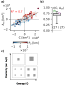
\includegraphics{scatter_and_box_cz_alt.pdf}
    \caption{.. Schematic of the relationship between the number, $N$, 
    and mean area of heavy precipitation features, $A_m$, 
    and coverage of heavy precipitation, $C$ (c). 
    $A_m$ increase from bottom left to top right panel, $N$ decrease from bottom right to top left panel, 
    and a spatial clustering in this framework is interpreted as increasing $A_m$ for a given $C$, denoted $A_m|C$.}
\label{spatial_preference_obsMAP}
\end{figure}

Since $N$ is a commonly used metric for quantifying clustering, we highlight that interpretations of clustering will be affected by whether clustering is considered to 
exhibit high degree of clustering for low- or high total area coverage (lines: 416-420), and that we interpret an increase in $C$ as an increased temporal clustering of heavy rainfall (lines: 12-14, 237-239).

\clearpage
\begin{itemize}
    \item Justification or sensitivity testing for the 5\% rainfall threshold
\end{itemize}
The purpose of the threshold is to isolate rainfall associated with strong convection, 
partly controlling for direct thermodynamic changes to rainfall with warming.
Early in this work we have explored 3\%, 5\% and 10\% thresholds, and during this revision all figures from the paper have been reproduced with these thresholds.
The overall conclusions from the paper are not sensitivie to the threshold, including;
uniform increase in $A_m$ with warming, 
generally increased proximity of heavy precipitation to the equator and hydrological equator with warming, 
El Ni\~no conditions associated with increased clusterng in interannual variability and with warming, 
and discrepencies between modelled and observed relative humidity and cloud signatures associated with clustering in interannual variability.  
Differences include, when using the top 10\%, the drying associated with $C$ in interannual variability is weaker and not statistically significant, instead Am$|$$C$ is associated with a drier tropics when using this threshold.
Further, the $C_z$ (now $P_z$ and increasing with increasing proximity $(-\infty, 0]$, to simplify interpretation of signs of correlations) relationship with $A_m$ for climatological change with warming is absent when using the top 10\%. 
When using the top 3\% the proximity to the hydrological equator, $C_{heq}$ (now $P_{heq}$) and $Pz$ explain close to 20\% of the variance each in $A_m$ with warming, where $P_{heq}$ is anticorrelated with changes in $A_m$. 
This was not a surprise, as $P_z$ and $P_{heq}$ are somewhat anticorrelated when using the top 5\% threshold. The revised manuscript mentions the testing, robustness, and caveats to using different thresholds 
(line: 194-196, line: 549-557).

\subsubsection*{2. Focus the title more specifically on the scope of the article}
We have changed the title to focus on the central question of the investigation (line: 1-2).
\clearpage


\subsection*{Specific comments}
\subsubsection*{Abstract}
\begin{itemize}
    \item Highlight motivation, main method, key findings, and implications without overgeneralizations
\end{itemize}
The abstract has been edited to a more objective summary (lines: 7-28).


\subsubsection*{Introduction}
\begin{itemize}
    \item Lacks a clear statement of research question and novelty
\end{itemize}
In the revised manuscript we have included a statement of the research question and novelty in the final paragraph of the introduction (lines: 112-127).

\begin{itemize}
    \item Lacks a clear statement of research gaps
\end{itemize}
The edited version of the final paragrah of the introduction also includes a statement of research gaps in existing literature, as it relates to large-scale clustering (lines: 112-127).


\subsubsection*{Data and Methods}
\begin{itemize}
    \item A percentile threshold on "heavy precipitation" may distort physical interpretation, since heavy precipitation areas vary seasonally and regionally.
\end{itemize}
We have added comments on the limitations of such a threshold in the conclusion (lines: 669-674).

\begin{itemize}
    \item Uncertainty estimates or sensitivity analysis, including robustness to detrending method and SST indices.
\end{itemize}
We have added p-values to the climatological model-spread scatters (Figure 5, 9, 11, 15), and an explanation of the method to consider correlations and linear regression statistically signficant (lines: 245-251).
Further, we have calculated correlations when potential model outliers are excluded (lines: 249-251 , lines: 598-600).
Regarding the detrending method, correlations of interannual variability are robust to whether the data is detrended or not (lines: 230-231). 
We decided to detrend the data for a closer comparison with the method applied for statistical analysis of clustering and radiative feedbacks in internnual variability by Bony et al. 2020.
In the paper, we have presented results for the ONI SST index to highlight El Ni\~no like conditions.
In the revised manuscript we have included a more atmospheric based El Ni\~no index, the Southern Oscillation Index (SOI), which shows similar relationships (lines: 374-384, Figure 8 and Figure S1 in supporting information).  
Regarding normalization of changes in temperature with warming, the results are similar for when using land and ocean or only ocean points. 

\begin{itemize}
    \item This section would benefit from a schematic of how $A_m$, $C$, $P_z$, $C_m$ (now $P_{eq}$) are related
\end{itemize}
We have included a figure (Figure 4 in the revised manuscript, Figure 2 below) with a schematic of how $P_z$, $P_{eq}$, and $P_{heq}$ are calculated, and how they relate to $A_m$ for a given $C$.

\begin{figure}[H]
    \centering
    \includegraphics{cz_cm_cheq_alt.pdf}    
    \caption{Schematic of metric and boxplot of its partial correlations with $A_m$ outside the influence of $C$, for $P_z$ (a), $P_{eq}$ (b), $P_{heq}$ (c)
    in the CMIP6 ensemble. The fraction of CMIP models with statistically significant correlations is indicated below each box, 
    and the GPCP (star) and high-resolution GCM (diamond) correlations are shown in lighter colors if not statistically significant.}
\label{spatial_preference_cz_cm_cheq}
\end{figure}

\begin{itemize}
    \item Discuss limited period of IFS\_FESOM
\end{itemize}
In terms of statistical robustness, the timeperiod of the data from the IFS\_FESOM model is the same as the observational data record used (25 years), where 5 years of spin-up is excluded.
Therefore, we believe we are justified in analysing interannual variability in the IFS\_FESOM model in an analogous way to the observations and CMIP models.
% We have added a comment about different high-resolution runs exhibiting quite different behaviours depending on the model set-up, and for that reason this particular model may not be 
% representative of high-resolution models overall.

\clearpage
\subsubsection*{Spatial Patterns and Variability}
\begin{itemize}
    \item What is the physical rationale for controlling for the total area covered by heavy rainfall? (Does $C$ correspond to an energetic constraints)
\end{itemize}
In interannual variability, the total area covered by heavy rainfall is most closely related to the domain-mean temperature and rainfall, which in turn has a strong effect on the environment radiative fluxes.
In this work, we primarily view total area covered by heavy precipitation, $C$, as a confounding variable and temporal clustering of rainfall, while $A_m$ for a given $C$ represents the spatial 
clustering, or organization of the existing amount of precipitation. Between climates, the timescale is long enough that changes in mean rainfall can be viewed as an energetic constraint on tropical precipitation area fraction, 
controlling for the direct thermodynamic changes in mean rainfall from CC-scaling of specific humidity. We have added description of the relationship between mean precipitation and total area coverage of heavy precipitation 
throughout the revised paper (lines: 15-17, lines: 232-239, lines: 549-557, lines: 669-672).

\clearpage
\subsubsection*{SST controls}
\begin{itemize}
    \item Highlight the distinction between relationships of internal variability and (ENSO-driven) and due to forced responses (warming induced SST patterns).
\end{itemize}
The text has been edited throughout, to highlighting that one form of relationship is a forced response to global warming, and the other natural variability (lines: 112-114, lines: 319-321, lines: 459-464, lines: 627-929)

\begin{itemize}
    \item Discuss causality: is clustering a response to SST anomalies, or does it feedback onto them via radiative effects?
\end{itemize}
To answer this question, we have included analysis of top of the atmosphere radiative fluxes from CERES-SYN1deg-Day regressed onto large-scale clustering in all-, clearsky-, and cloudy conditions.
The results suggest that cloud-radiative and clear-sky feedbacks may act to feedback on the spatial pattern of heavy rainfall associated with highly clustered states and El Ni\~no conditions
(Figure S7 in supporting information and lines: 157-158, lines: 633-638).

\begin{itemize}
    \item Clarify how surface tempearture is used and include regression strength.
\end{itemize}
The surface temperature ($T_s$) includes both land and ocean. We have edited figure descriptions and text to clarify (lines: 390-391, Figure 5 description, Figure 7 description).
We have added p-values to the climatological model-spread scatter and an explanation of the method to consider correlations and linear regression statistically signficant (lines: 245-251).

\begin{itemize}
    \item Consider rewording "changes in large-scale clustering with warming have little connection to changes in the tropical-mean RH and low-cloud fraction" to a less general statement and include a correlation matrix of the model-ensemble 
    correlations with relative humidity and low cloudiness.
\end{itemize}
We have changed this line to clarify that we mean based on the perspective of overall clustering of heavy precipitation that we take in this investigation (lines 564-568).
The appendix includes a summary of the relationships between different clustering measures and radiative feedback metrics (Figure S2 in supporting information) (lines: 493-496, lines: 588-590).

\begin{itemize}
    \item More concise description of Figure 10-12: Why does the observed RH changes vanish after controlling for $C$, while model behaviour diverges. 
\end{itemize}
We have included the relationships between the radiative feedback metrics and $C$ in these figures, and added description of one possible reason why observations and models diverge in this way (lines: 549-557).

\begin{itemize}
    \item Include robustness test of relationship for projected relative drying with increasing proximity of heavy rainfall to the equator.
\end{itemize}
We have included a robustness test by removing potential model outliers, and the result is that the relationship vanish when these models are removed (lines: 599-601).

\clearpage
\subsubsection*{Summary and Discussion}
\begin{itemize}
    \item Summmary needs a critical evaluation of uncertainties
\end{itemize}
In the paragraph covering the limitations of the methodology we include;
limitations of the representation of convection and heavy rainfall in GCMs, 
the limitations of inferring statistical relationships from a relatively small set of models with at times diverging clustering behaviour in more than one way (interannual, climatological, and/or for tendency with global warming),
and what conclusions we feel more confident in.
We have added a discussion about the limitations in the methodology of using a percentile threshold for identifying heavy rainfall  

\begin{itemize}
    \item Consider tempering statements about effects on radiative feedbacks and ECS
\end{itemize}
We have included clarification that we are referring to large-scale clusterng from the perspective of clustering taken in this investigation (lines: 572-575).

\begin{itemize}
    \item Consider schematic emphasizing key mechanisms (clustering of heavy precipitation, SST gradient, ITCZ narrowing, and humidity/cloud response)
\end{itemize}
"Not sure what to say here, but I feel like this might be hard to do at this point"


\end{document}







% Figure 1 shows more clearly the precipitation field, heavily precipitating points, and the precipitation features (8-connected components).
% \begin{figure}
%     \centering
%     \includegraphics{example_plot.pdf}
%     \caption{February daily snapshots of GPCP precipitation (blue colors) and heavy precipitation (black shading) features (red contour), 
%     with monthly specific humidity representing the median over the tropics (black contour). 
%     The panel titles show the total area coverage of heavy precipitation, $C$, and the mean area of precipitation features, $A_m$, with
%     the proximity of heavily precipitation points to the central pacific, equator, and hydrological equator below
%     (described in greater detail in Figure 4).
%     }
% \label{spatial_preference_exampleMAPS}
% \end{figure}



